\documentclass{article}\usepackage[]{graphicx}\usepackage[]{color}
%% maxwidth is the original width if it is less than linewidth
%% otherwise use linewidth (to make sure the graphics do not exceed the margin)
\makeatletter
\def\maxwidth{ %
  \ifdim\Gin@nat@width>\linewidth
    \linewidth
  \else
    \Gin@nat@width
  \fi
}
\makeatother

\definecolor{fgcolor}{rgb}{0.345, 0.345, 0.345}
\newcommand{\hlnum}[1]{\textcolor[rgb]{0.686,0.059,0.569}{#1}}%
\newcommand{\hlstr}[1]{\textcolor[rgb]{0.192,0.494,0.8}{#1}}%
\newcommand{\hlcom}[1]{\textcolor[rgb]{0.678,0.584,0.686}{\textit{#1}}}%
\newcommand{\hlopt}[1]{\textcolor[rgb]{0,0,0}{#1}}%
\newcommand{\hlstd}[1]{\textcolor[rgb]{0.345,0.345,0.345}{#1}}%
\newcommand{\hlkwa}[1]{\textcolor[rgb]{0.161,0.373,0.58}{\textbf{#1}}}%
\newcommand{\hlkwb}[1]{\textcolor[rgb]{0.69,0.353,0.396}{#1}}%
\newcommand{\hlkwc}[1]{\textcolor[rgb]{0.333,0.667,0.333}{#1}}%
\newcommand{\hlkwd}[1]{\textcolor[rgb]{0.737,0.353,0.396}{\textbf{#1}}}%

\usepackage{framed}
\makeatletter
\newenvironment{kframe}{%
 \def\at@end@of@kframe{}%
 \ifinner\ifhmode%
  \def\at@end@of@kframe{\end{minipage}}%
  \begin{minipage}{\columnwidth}%
 \fi\fi%
 \def\FrameCommand##1{\hskip\@totalleftmargin \hskip-\fboxsep
 \colorbox{shadecolor}{##1}\hskip-\fboxsep
     % There is no \\@totalrightmargin, so:
     \hskip-\linewidth \hskip-\@totalleftmargin \hskip\columnwidth}%
 \MakeFramed {\advance\hsize-\width
   \@totalleftmargin\z@ \linewidth\hsize
   \@setminipage}}%
 {\par\unskip\endMakeFramed%
 \at@end@of@kframe}
\makeatother

\definecolor{shadecolor}{rgb}{.97, .97, .97}
\definecolor{messagecolor}{rgb}{0, 0, 0}
\definecolor{warningcolor}{rgb}{1, 0, 1}
\definecolor{errorcolor}{rgb}{1, 0, 0}
\newenvironment{knitrout}{}{} % an empty environment to be redefined in TeX

\usepackage{alltt}
\usepackage[margin=1in,landscape]{geometry}
\usepackage{amsmath}
\usepackage{amsthm}
\usepackage{graphicx,psfrag,epsf}
\renewcommand{\thefigure}{S\arabic{figure}}

\title{Supplementary materials for \textit{Small sample methods for cluster-robust variance estimation and hypothesis testing in fixed effects models}}
\author{James E. Pustejovsky \& Elizabeth Tipton}
\IfFileExists{upquote.sty}{\usepackage{upquote}}{}
\begin{document}
\maketitle




\begin{knitrout}
\definecolor{shadecolor}{rgb}{0.969, 0.969, 0.969}\color{fgcolor}\begin{figure}

{\centering 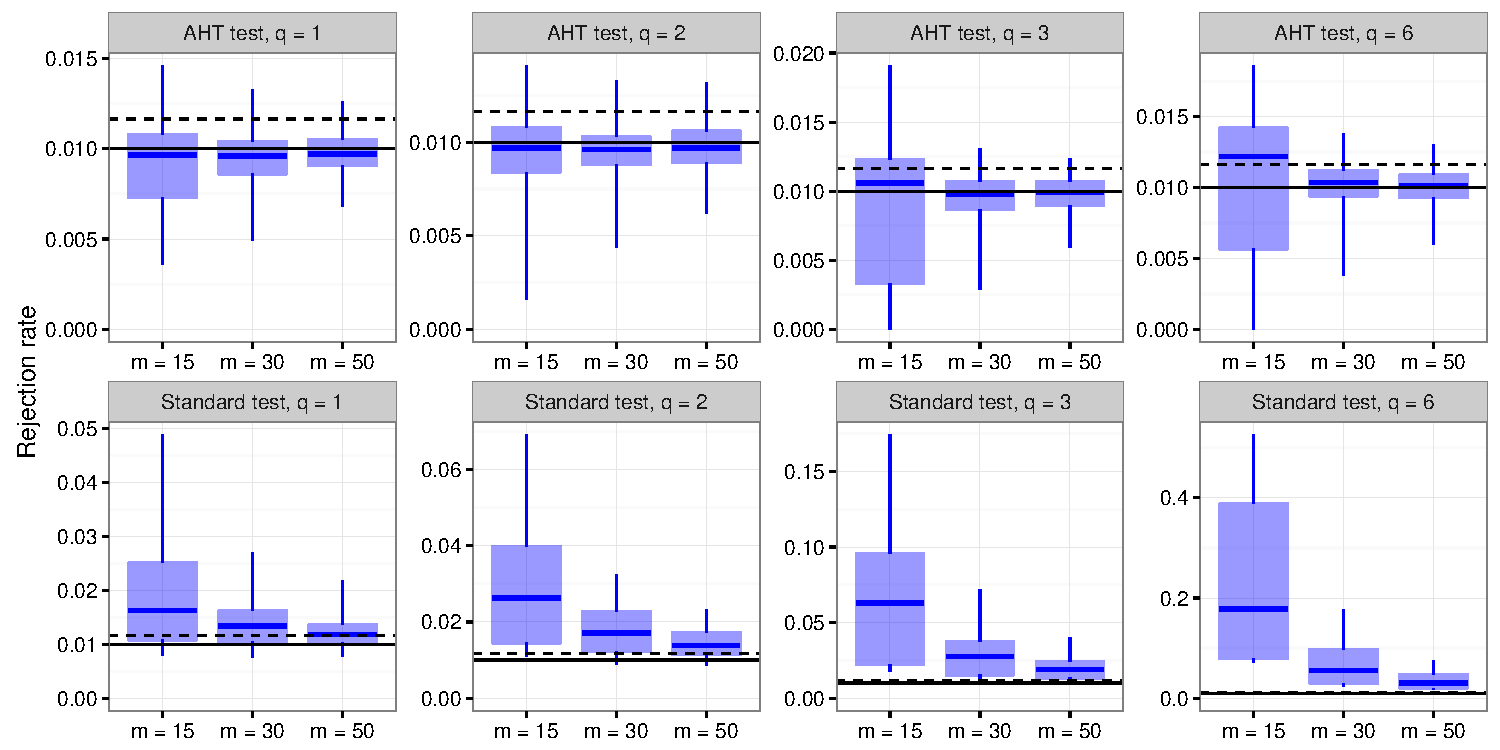
\includegraphics[width=\linewidth]{CR_fig/overview_01-1} 

}

\caption[Rejection rates of AHT and standard tests for ]{Rejection rates of AHT and standard tests for $\alpha = .01$, by dimension of hypothesis ($q$) and sample size ($m$).}\label{fig:overview_01}
\end{figure}


\end{knitrout}

\begin{knitrout}
\definecolor{shadecolor}{rgb}{0.969, 0.969, 0.969}\color{fgcolor}\begin{figure}

{\centering 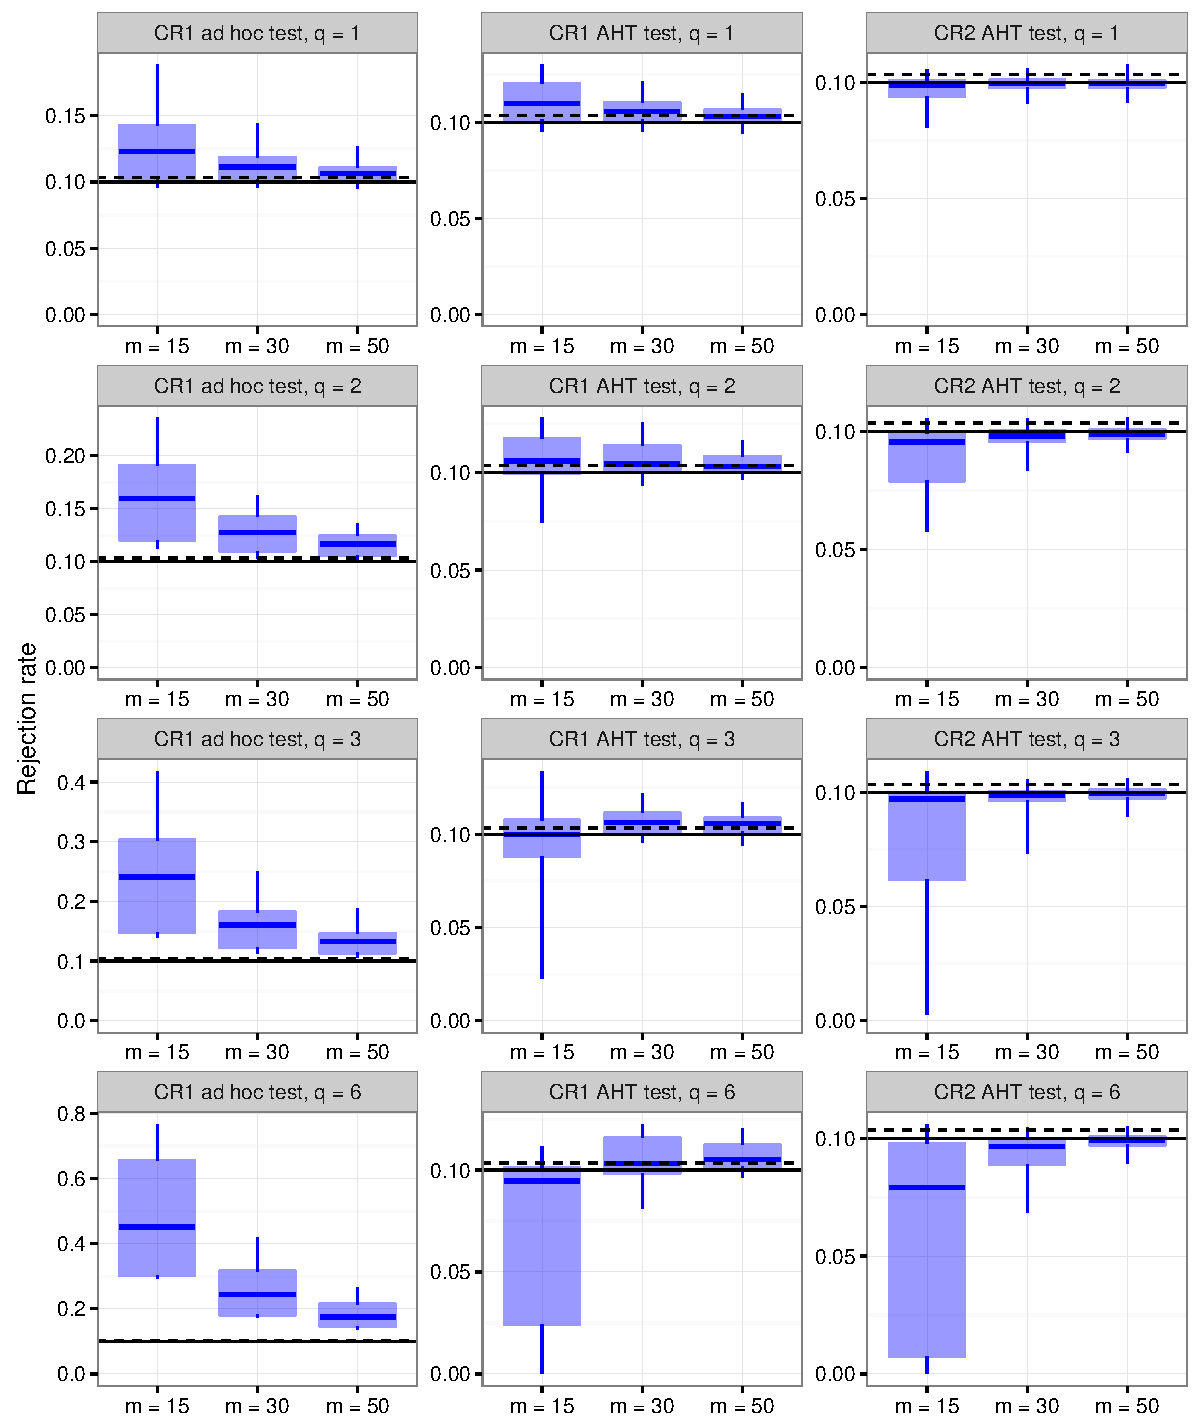
\includegraphics[width=\linewidth]{CR_fig/overview_10-1} 

}

\caption[Rejection rates of AHT and standard tests for ]{Rejection rates of AHT and standard tests for $\alpha = .10$, by dimension of hypothesis ($q$) and sample size ($m$).}\label{fig:overview_10}
\end{figure}


\end{knitrout}

\begin{knitrout}
\definecolor{shadecolor}{rgb}{0.969, 0.969, 0.969}\color{fgcolor}\begin{figure}

{\centering 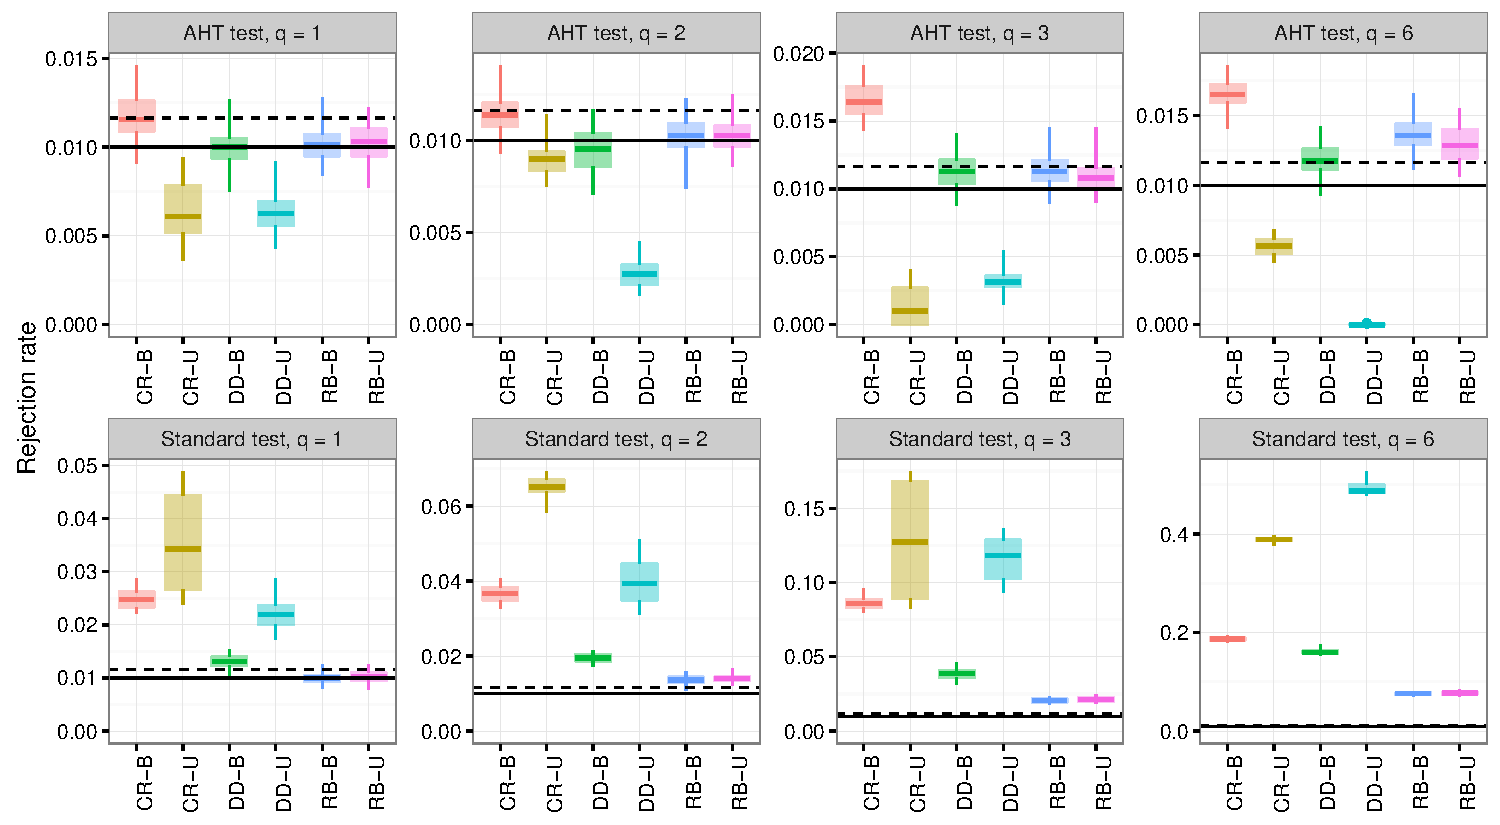
\includegraphics[width=\linewidth]{CR_fig/balance_01_15-1} 

}

\caption[Rejection rates of AHT and standard tests, by study design and dimension of hypothesis (]{Rejection rates of AHT and standard tests, by study design and dimension of hypothesis ($q$) for $\alpha = .01$ and $m = 15$. CR = cluster-randomized design; DD = difference-in-differences design; RB = randomized block design; B = balanced; U = unbalanced.}\label{fig:balance_01_15}
\end{figure}


\end{knitrout}

\begin{knitrout}
\definecolor{shadecolor}{rgb}{0.969, 0.969, 0.969}\color{fgcolor}\begin{figure}

{\centering 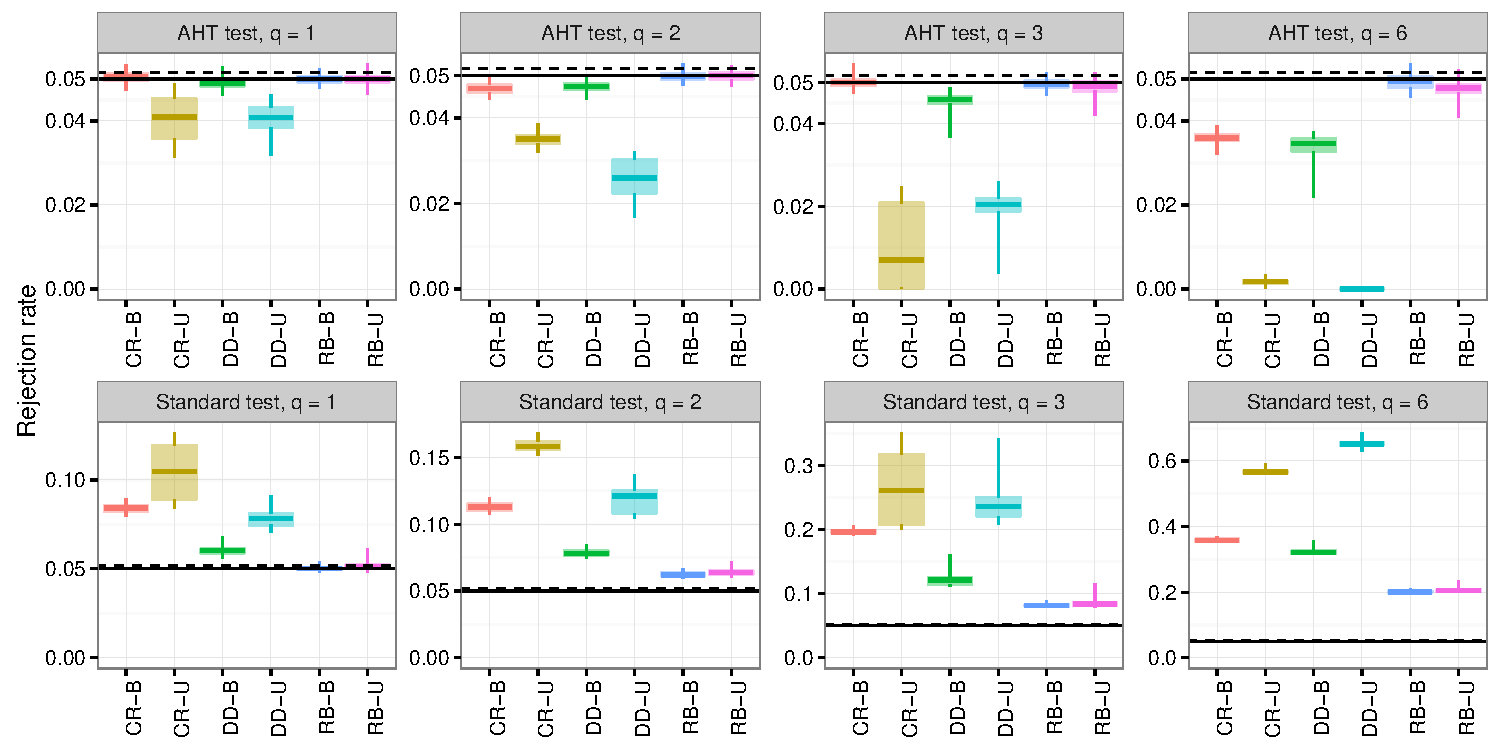
\includegraphics[width=\linewidth]{CR_fig/balance_05_15-1} 

}

\caption[Rejection rates of AHT and standard tests, by study design and dimension of hypothesis (]{Rejection rates of AHT and standard tests, by study design and dimension of hypothesis ($q$) for $\alpha = .05$ and $m = 15$. CR = cluster-randomized design; DD = difference-in-differences design; RB = randomized block design; B = balanced; U = unbalanced.}\label{fig:balance_05_15}
\end{figure}


\end{knitrout}

\begin{knitrout}
\definecolor{shadecolor}{rgb}{0.969, 0.969, 0.969}\color{fgcolor}\begin{figure}

{\centering 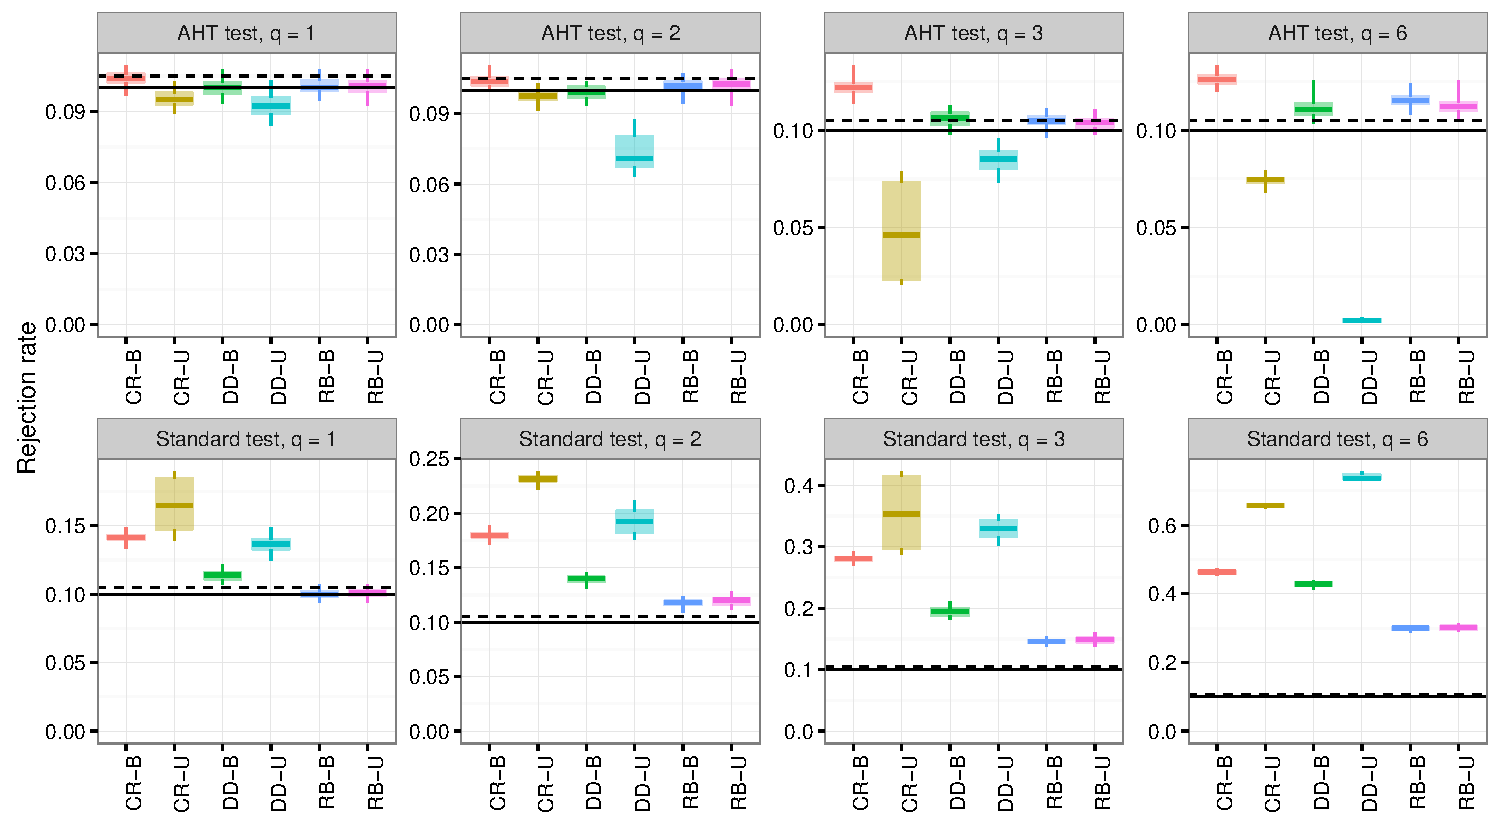
\includegraphics[width=\linewidth]{CR_fig/balance_10_15-1} 

}

\caption[Rejection rates of AHT and standard tests, by study design and dimension of hypothesis (]{Rejection rates of AHT and standard tests, by study design and dimension of hypothesis ($q$) for $\alpha = .10$ and $m = 15$. CR = cluster-randomized design; DD = difference-in-differences design; RB = randomized block design; B = balanced; U = unbalanced.}\label{fig:balance_10_15}
\end{figure}


\end{knitrout}

\begin{knitrout}
\definecolor{shadecolor}{rgb}{0.969, 0.969, 0.969}\color{fgcolor}\begin{figure}

{\centering 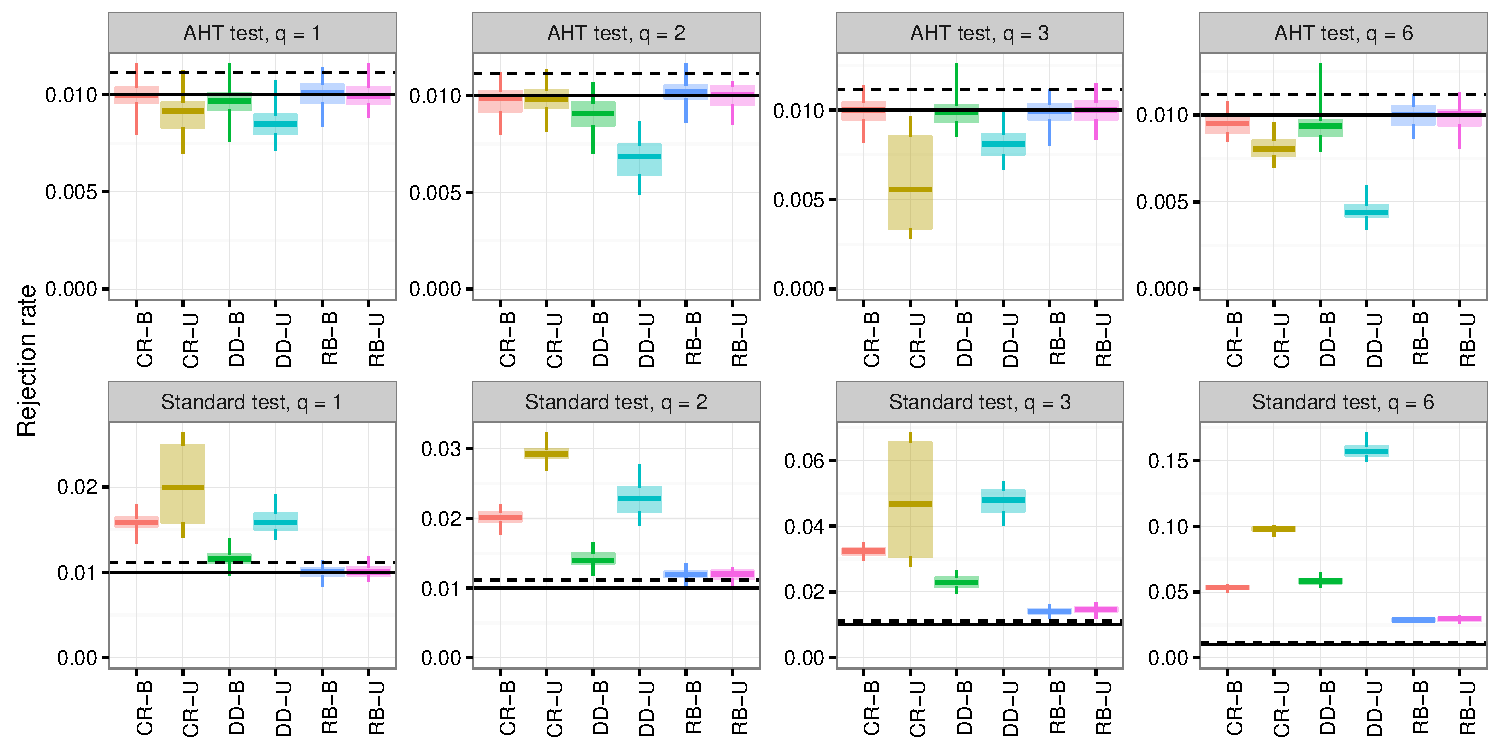
\includegraphics[width=\linewidth]{CR_fig/balance_01_30-1} 

}

\caption[Rejection rates of AHT and standard tests, by study design and dimension of hypothesis (]{Rejection rates of AHT and standard tests, by study design and dimension of hypothesis ($q$) for $\alpha = .01$ and $m = 30$. CR = cluster-randomized design; DD = difference-in-differences design; RB = randomized block design; B = balanced; U = unbalanced.}\label{fig:balance_01_30}
\end{figure}


\end{knitrout}

\begin{knitrout}
\definecolor{shadecolor}{rgb}{0.969, 0.969, 0.969}\color{fgcolor}\begin{figure}

{\centering 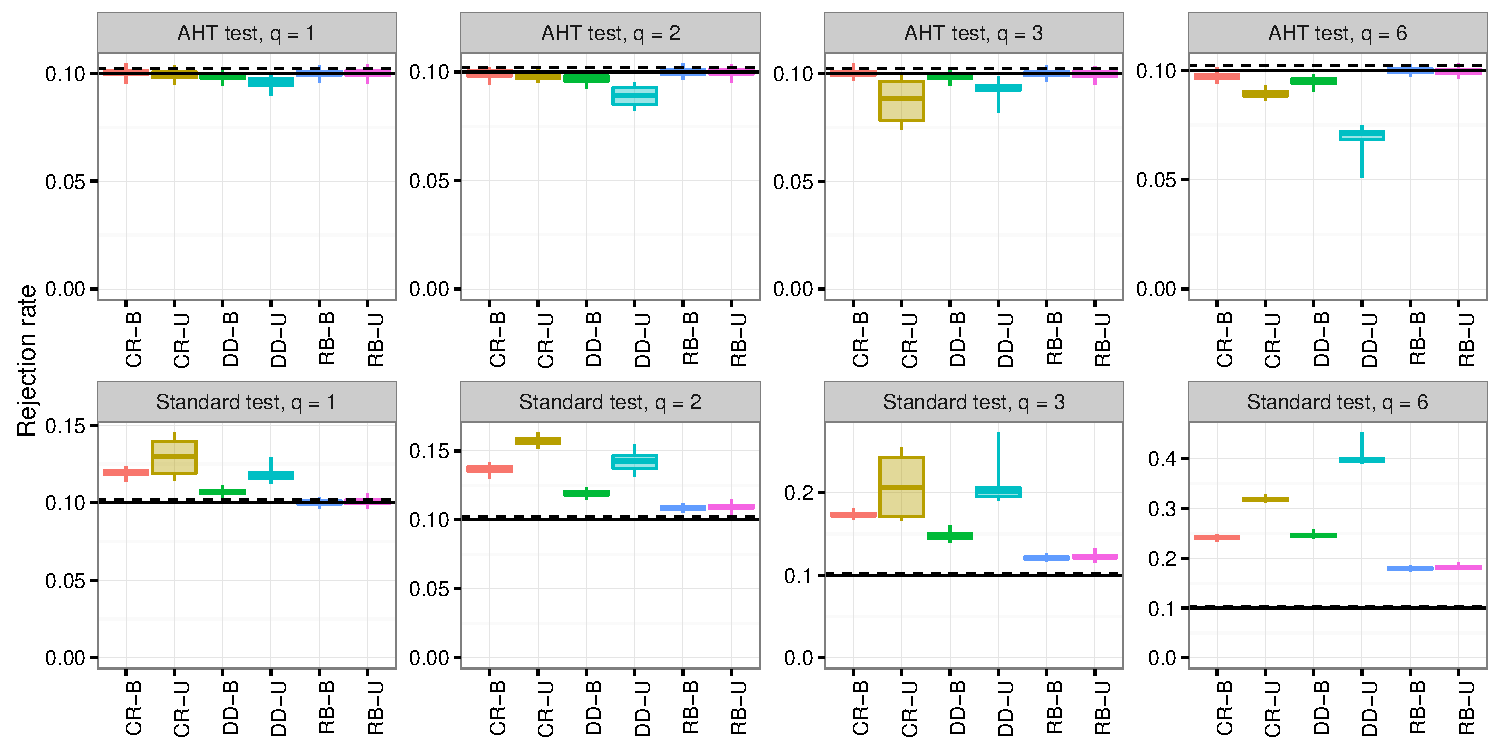
\includegraphics[width=\linewidth]{CR_fig/balance_10_30-1} 

}

\caption[Rejection rates of AHT and standard tests, by study design and dimension of hypothesis (]{Rejection rates of AHT and standard tests, by study design and dimension of hypothesis ($q$) for $\alpha = .10$ and $m = 30$. CR = cluster-randomized design; DD = difference-in-differences design; RB = randomized block design; B = balanced; U = unbalanced.}\label{fig:balance_10_30}
\end{figure}


\end{knitrout}

\begin{knitrout}
\definecolor{shadecolor}{rgb}{0.969, 0.969, 0.969}\color{fgcolor}\begin{figure}

{\centering 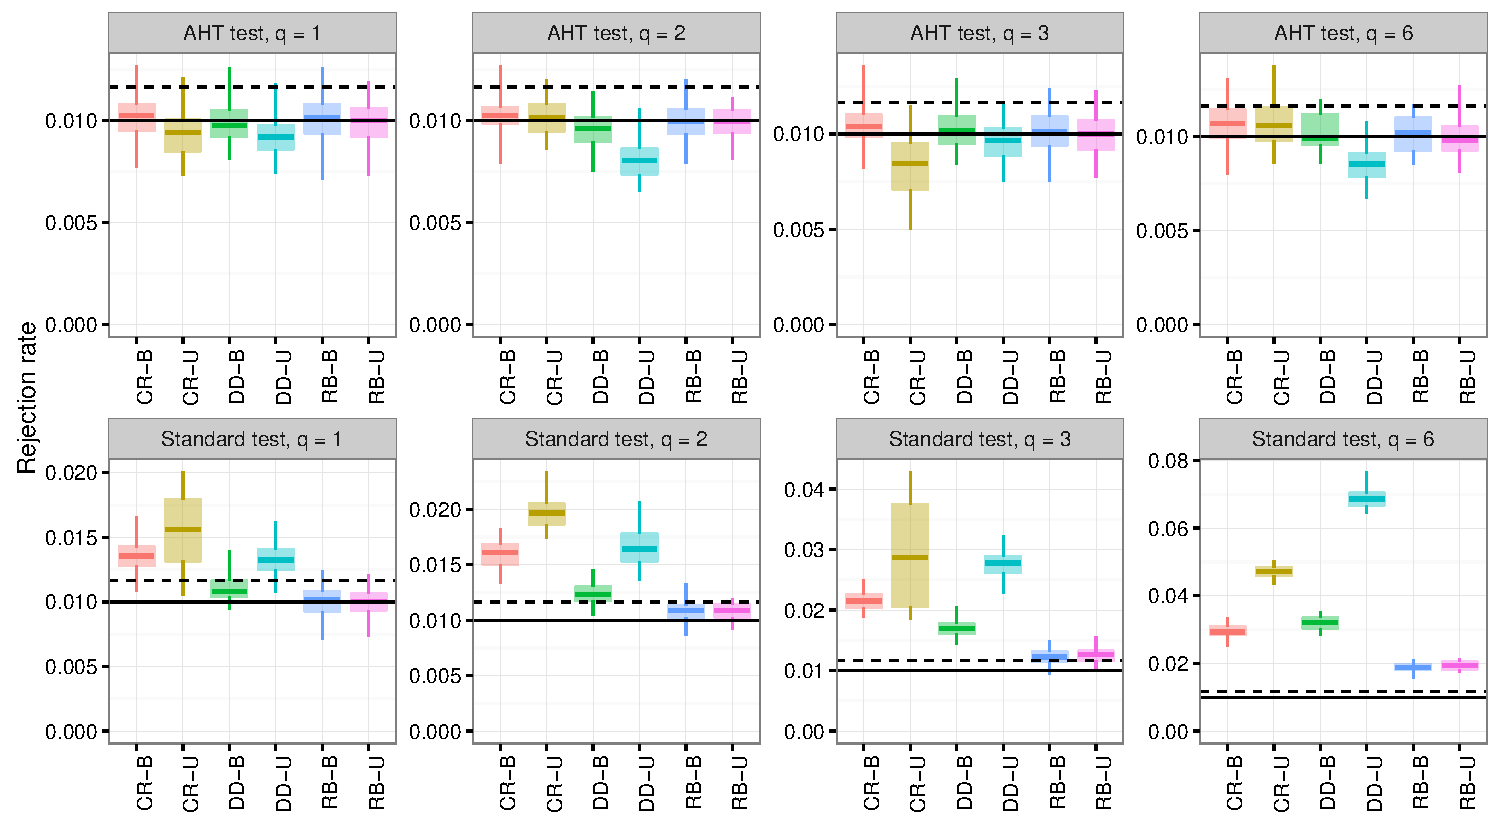
\includegraphics[width=\linewidth]{CR_fig/balance_01_50-1} 

}

\caption[Rejection rates of AHT and standard tests, by study design and dimension of hypothesis (]{Rejection rates of AHT and standard tests, by study design and dimension of hypothesis ($q$) for $\alpha = .01$ and $m = 50$. CR = cluster-randomized design; DD = difference-in-differences design; RB = randomized block design; B = balanced; U = unbalanced.}\label{fig:balance_01_50}
\end{figure}


\end{knitrout}

\begin{knitrout}
\definecolor{shadecolor}{rgb}{0.969, 0.969, 0.969}\color{fgcolor}\begin{figure}

{\centering 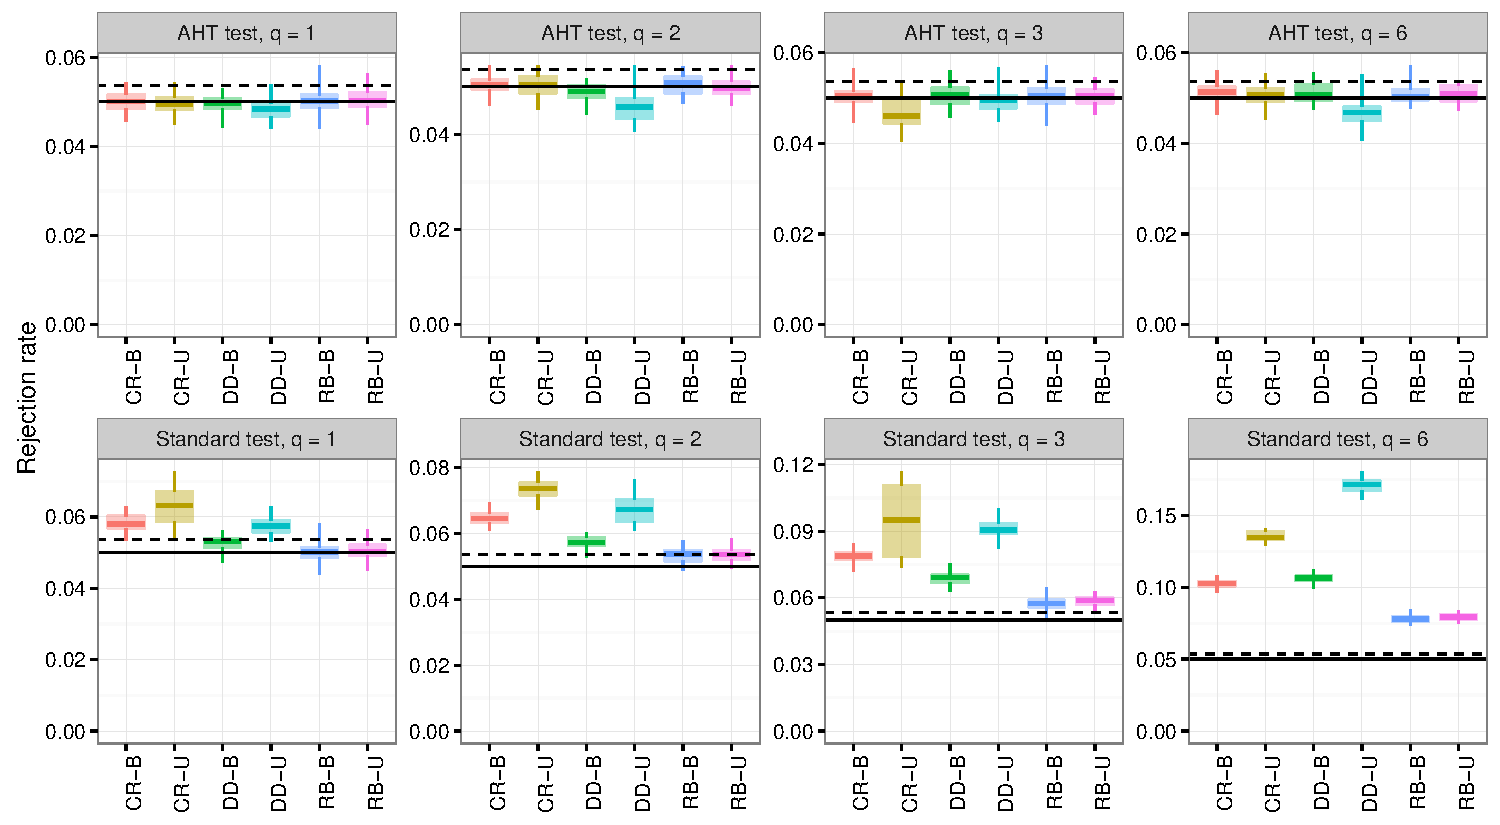
\includegraphics[width=\linewidth]{CR_fig/balance_05_50-1} 

}

\caption[Rejection rates of AHT and standard tests, by study design and dimension of hypothesis (]{Rejection rates of AHT and standard tests, by study design and dimension of hypothesis ($q$) for $\alpha = .05$ and $m = 50$. CR = cluster-randomized design; DD = difference-in-differences design; RB = randomized block design; B = balanced; U = unbalanced.}\label{fig:balance_05_50}
\end{figure}


\end{knitrout}

\begin{knitrout}
\definecolor{shadecolor}{rgb}{0.969, 0.969, 0.969}\color{fgcolor}\begin{figure}

{\centering 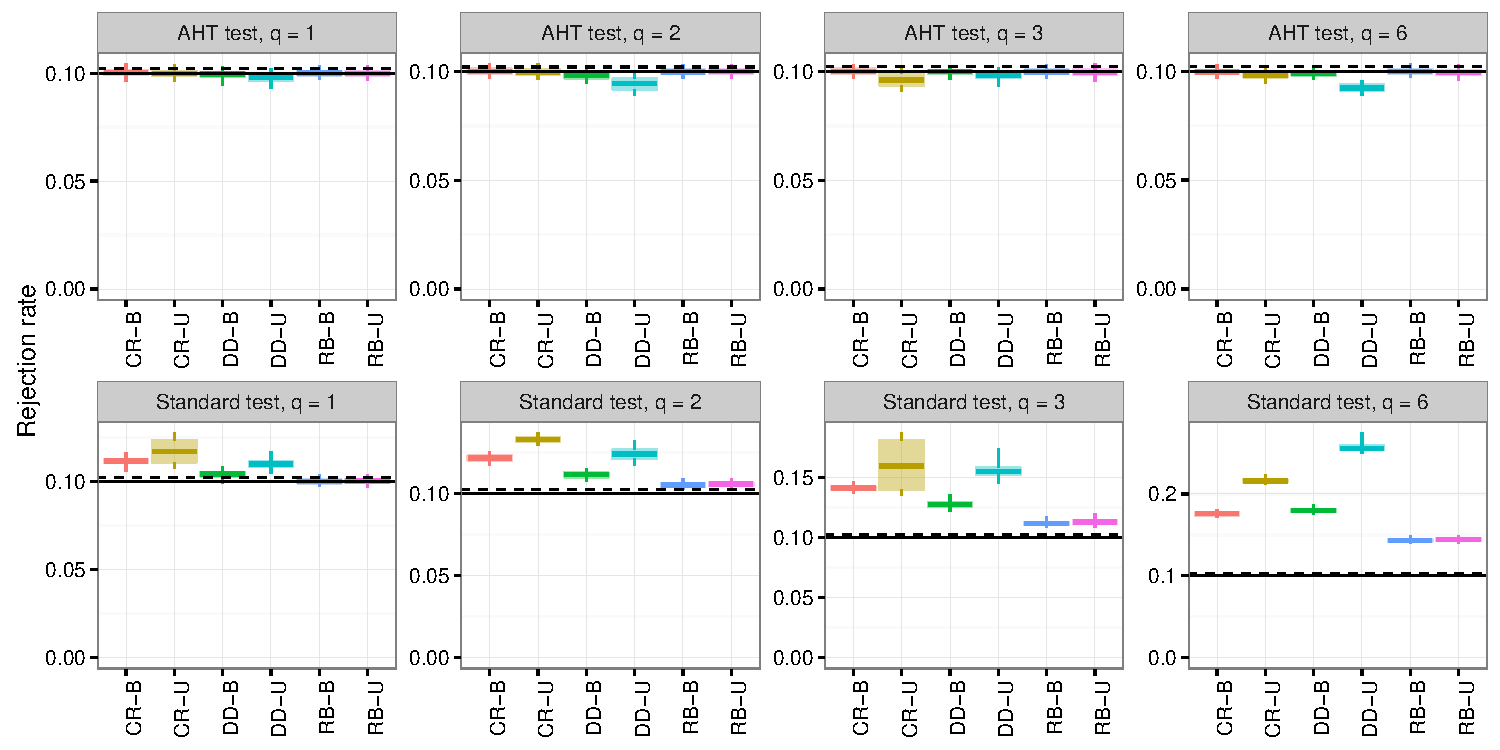
\includegraphics[width=\linewidth]{CR_fig/balance_10_50-1} 

}

\caption[Rejection rates of AHT and standard tests, by study design and dimension of hypothesis (]{Rejection rates of AHT and standard tests, by study design and dimension of hypothesis ($q$) for $\alpha = .10$ and $m = 50$. CR = cluster-randomized design; DD = difference-in-differences design; RB = randomized block design; B = balanced; U = unbalanced.}\label{fig:balance_10_50}
\end{figure}


\end{knitrout}

\begin{knitrout}
\definecolor{shadecolor}{rgb}{0.969, 0.969, 0.969}\color{fgcolor}\begin{figure}

{\centering 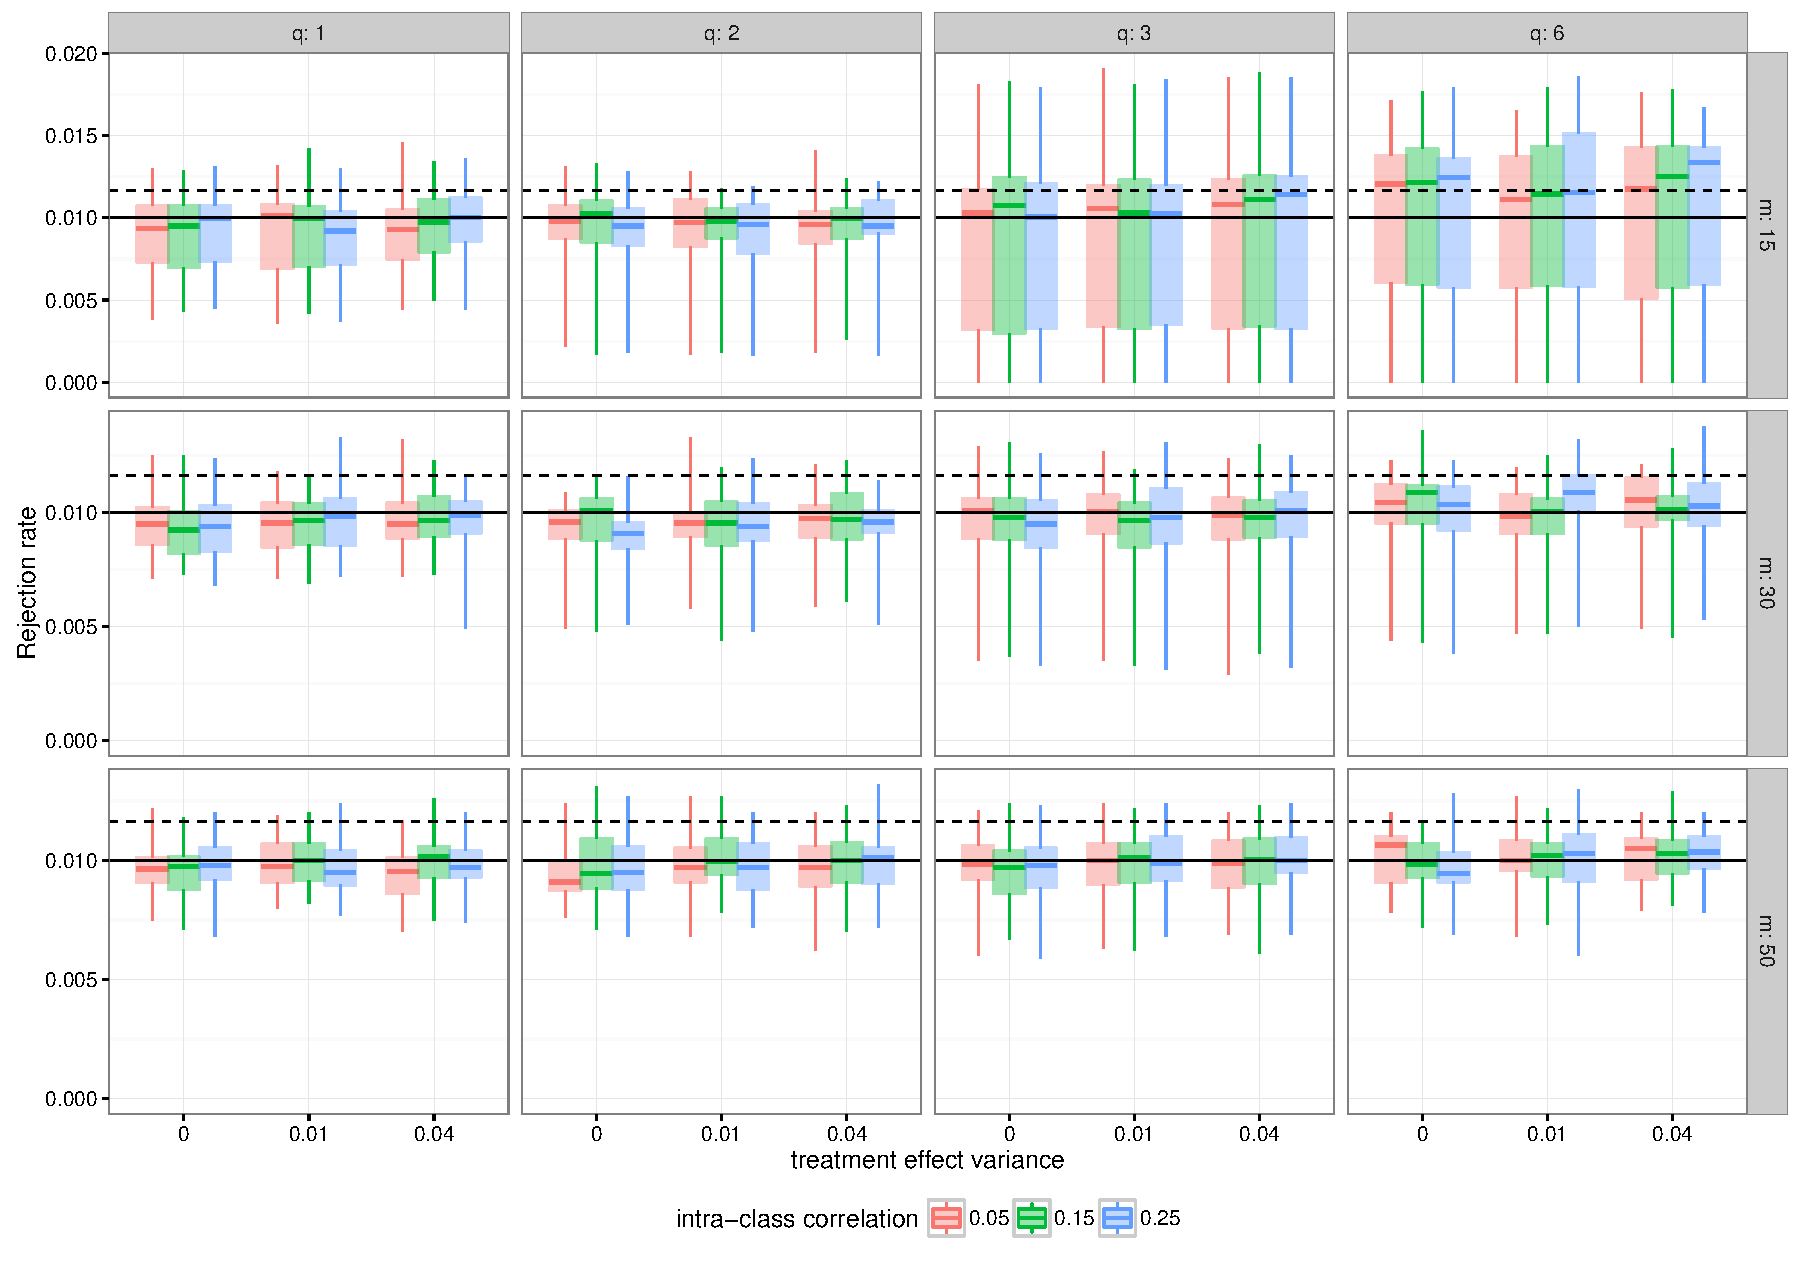
\includegraphics[width=\linewidth]{CR_fig/misspecification_01-1} 

}

\caption[Rejection rates of AHT test, by treatment effect variance and intra-class correlation for ]{Rejection rates of AHT test, by treatment effect variance and intra-class correlation for $\alpha = .01$.}\label{fig:misspecification_01}
\end{figure}


\end{knitrout}

\begin{knitrout}
\definecolor{shadecolor}{rgb}{0.969, 0.969, 0.969}\color{fgcolor}\begin{figure}

{\centering 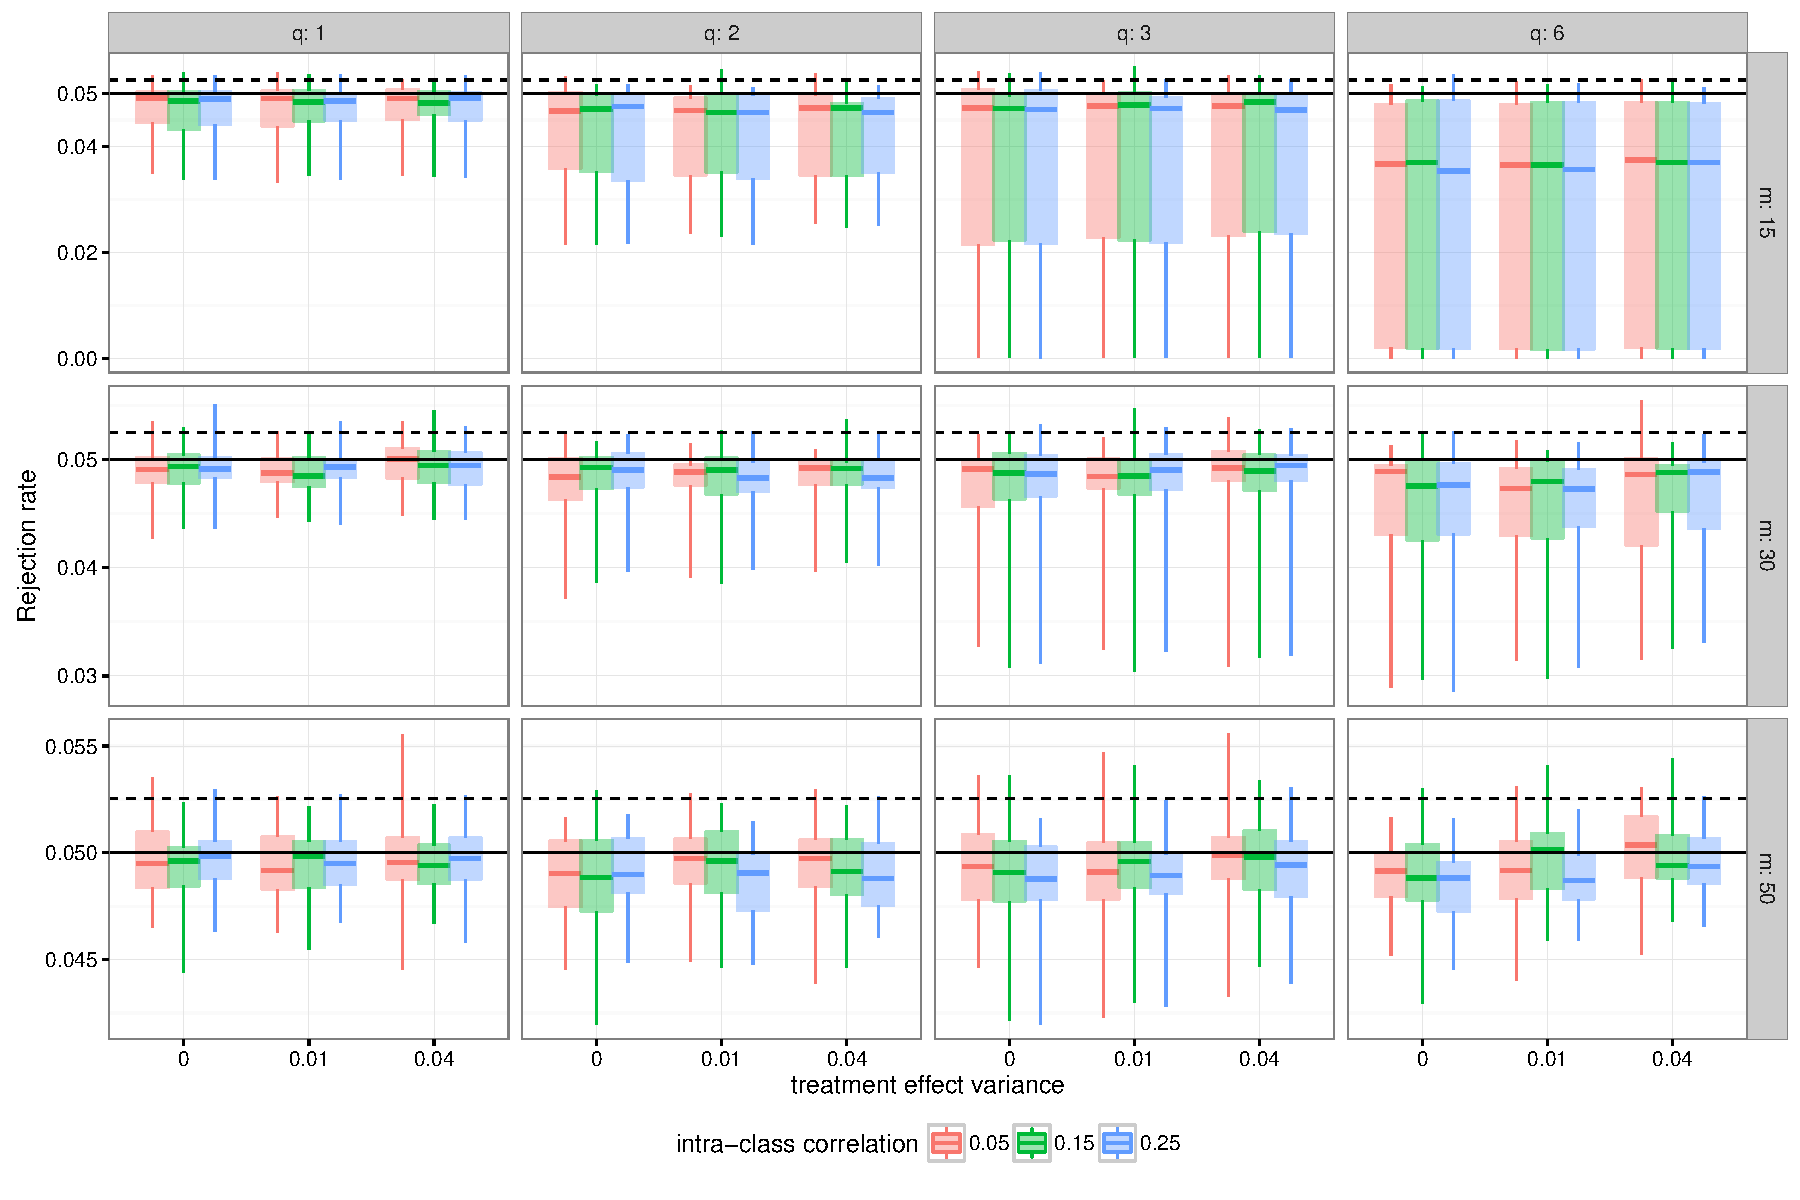
\includegraphics[width=\linewidth]{CR_fig/misspecification_05-1} 

}

\caption[Rejection rates of AHT test, by treatment effect variance and intra-class correlation for ]{Rejection rates of AHT test, by treatment effect variance and intra-class correlation for $\alpha = .05$.}\label{fig:misspecification_05}
\end{figure}


\end{knitrout}

\begin{knitrout}
\definecolor{shadecolor}{rgb}{0.969, 0.969, 0.969}\color{fgcolor}\begin{figure}

{\centering 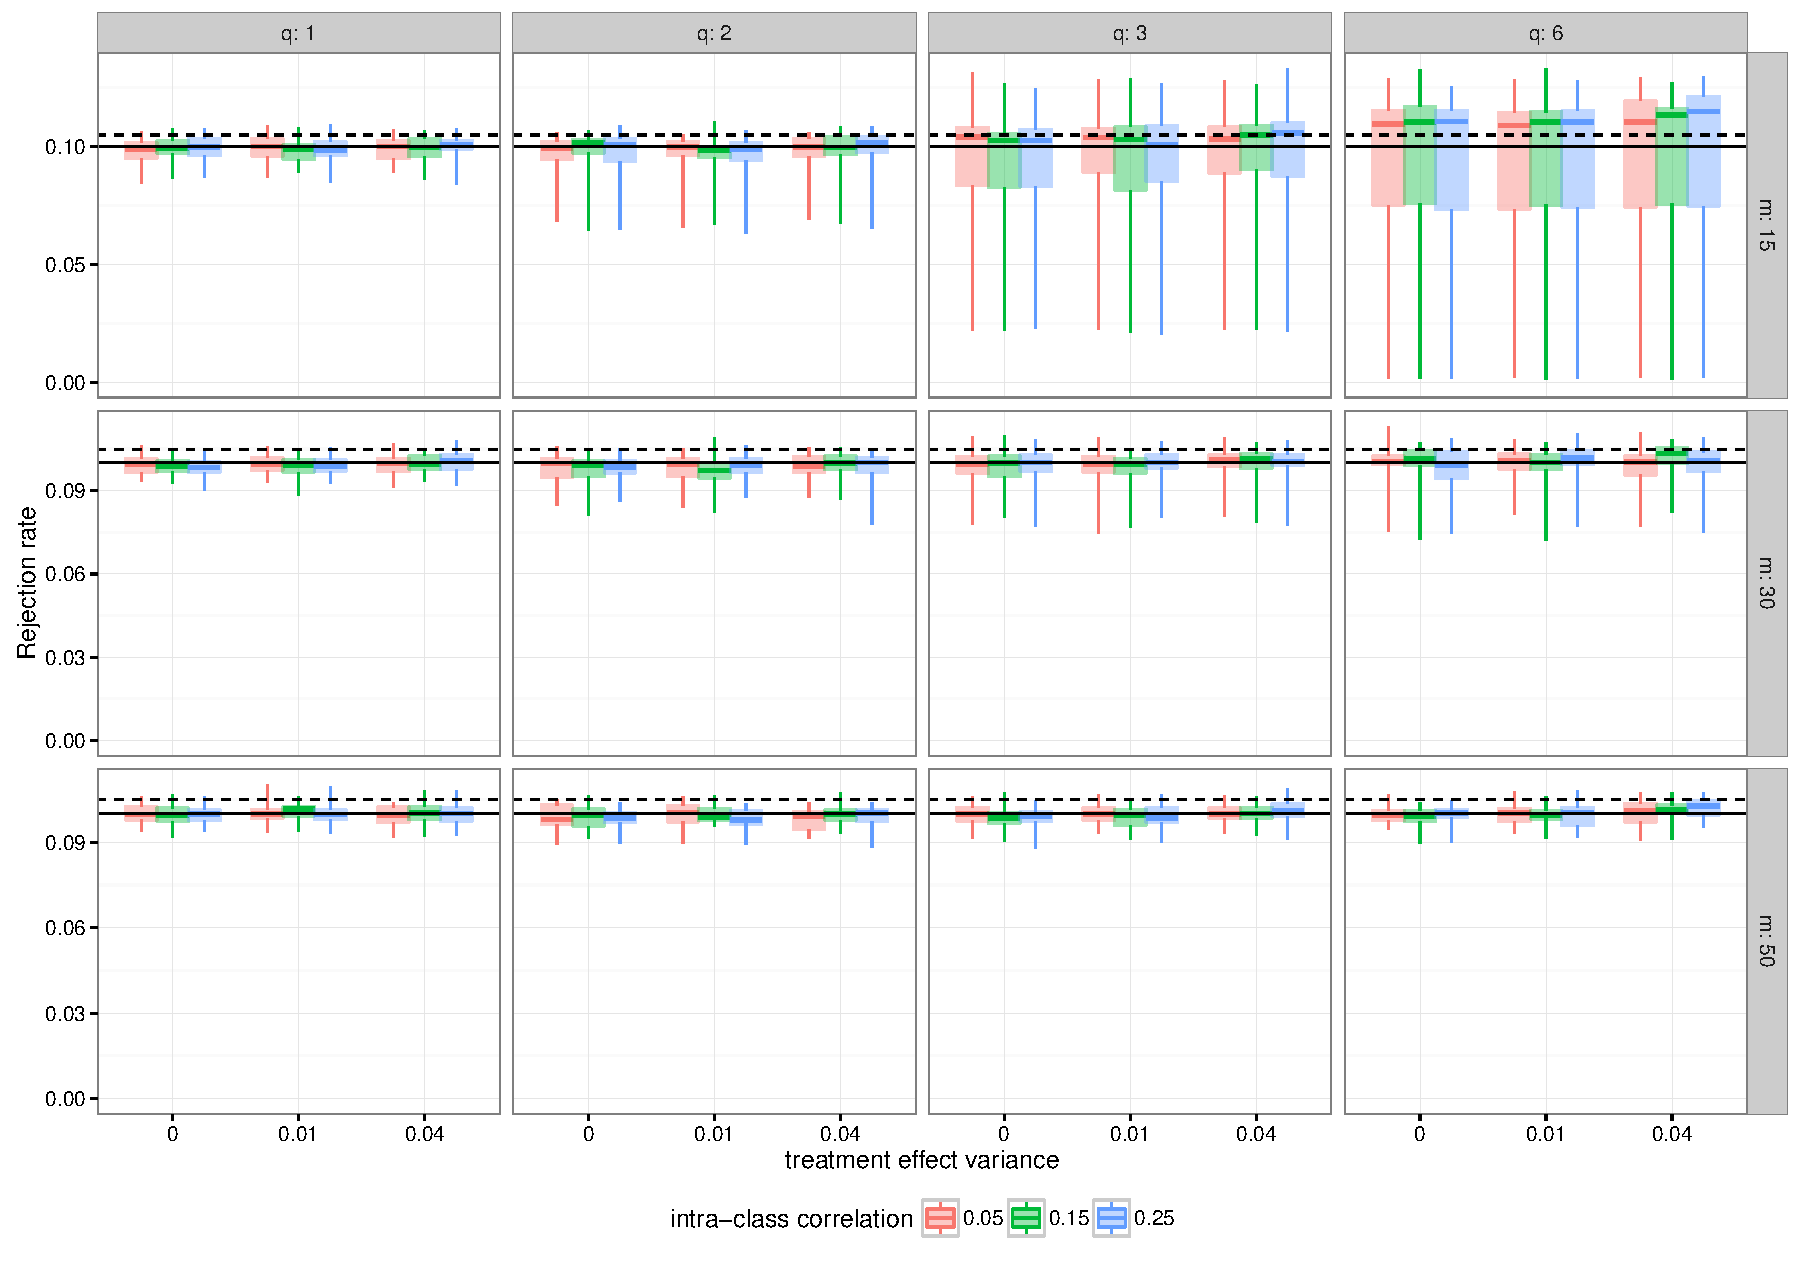
\includegraphics[width=\linewidth]{CR_fig/misspecification_10-1} 

}

\caption[Rejection rates of AHT test, by treatment effect variance and intra-class correlation for ]{Rejection rates of AHT test, by treatment effect variance and intra-class correlation for $\alpha = .10$.}\label{fig:misspecification_10}
\end{figure}


\end{knitrout}

\end{document}
